\documentclass[10.5pt,a4paper]{article}
\usepackage[margin=2cm]{geometry}
\usepackage{booktabs,graphicx,amsmath,amssymb,enumitem,xcolor,array,float,caption,tabularx}
\usepackage[hidelinks]{hyperref}
\setlist{nosep,leftmargin=1.4em}
\setlength{\parindent}{0pt}\setlength{\parskip}{4pt}
\captionsetup{font=small,labelfont=bf}
\newcommand{\fix}[1]{\textcolor{red}{\textbf{[#1]}}}
\newcommand{\RMSE}{\mathrm{RMSE}}

\begin{document}

\begin{center}
{\Large\bfseries AI651 Deep Learning for Space, Time and Graphs --- Programming Assignment 1}\\[4pt]
{\large Usama Azam \quad Roll no.\ 25280109 \quad \texttt{25280109@lums.edu.pk}}\\[4pt]
\textbf{GitHub repository (public):} \url{https://github.com/uazam1163-debug/AI651-PA1}\\[2pt]
{\small Task 1: executed full-preset notebook \texttt{Task1/Assignment1\_solved.ipynb}. Task 2: \texttt{Task2/} (v1 and v2 notebooks, declared $P$ and $E$).}
\end{center}

%=====================================================================
\section*{Task 1 --- Forecasting across heterogeneous sensors}

\textbf{Run.} \texttt{PA1\_PRESET=full}, data seed 0, model seed 0, Kaggle GPU (T4). All notebook checks passed.
Eligible origins: 650 train / 105 validation / 105 test. Implemented:
\begin{itemize}
\item \texttt{RawAttentionForecaster.forward}: circular Conv1d embedding $\to$ $+$ positions $\to$ 2 encoder blocks $\to$ LayerNorm $\to$ flatten $\to$ linear head ($[B,96,1]\to[B,48]$).
\item \texttt{SeriesDecomposition.forward}: centred moving average with \emph{replicate} padding (\texttt{avg\_pool1d}); returns (remainder, trend) with remainder $+$ trend $=x$.
\item \texttt{aggregate\_delays}: $z_t=\sum_j \alpha_j v_{(t-\tau_j)\bmod L}$ via an index tensor $(t-\tau_j)\bmod L$ and \texttt{gather}, per example, shared over heads/features (worked example gives $z_0=35$).
\end{itemize}
All numbers below are \emph{validation} unless marked \emph{test}; ``established'' = Stations 1--3, ``held-out'' = Station 4.

%---------------------------------------------------------------------
\subsection*{Response 1A --- predicted vs measured ordering}

\textbf{Expected ordering (written before Output 1.1)} \fix{confirm this was your own prior; edit if not}:
established: period-routed ridge $<$ Raw Attention $<$ sensor-specific ridge $\approx$ shared ridge;
held-out: period-routed ridge $<$ Raw Attention $<$ shared ridge (sensor-specific unavailable).
Reasoning: only routing and Attention can react to the operating pace; station identity does not determine the pace.

\begin{table}[H]\centering\small
\caption{Output 1.1 --- validation RMSE (m/s$^2$) by population and product.}
\begin{tabular}{lcccccccc}\toprule
& \multicolumn{4}{c}{Established (Stations 1--3)} & \multicolumn{4}{c}{Held-out (Station 4)}\\
\cmidrule(lr){2-5}\cmidrule(lr){6-9}
Model & All & A & B & C & All & A & B & C\\\midrule
Shared ridge & 0.767 & 0.805 & 0.854 & 0.621 & 0.876 & 0.909 & 0.982 & 0.713\\
Sensor-specific ridge & 0.768 & 0.804 & 0.852 & 0.630 & -- & -- & -- & --\\
Period-routed ridge & \textbf{0.166} & 0.181 & 0.164 & 0.152 & \textbf{0.173} & 0.184 & 0.182 & 0.150\\
Raw Attention & 0.427 & 0.424 & 0.448 & 0.407 & 0.667 & 0.707 & 0.629 & 0.662\\\bottomrule
\end{tabular}\end{table}

\begin{itemize}
\item \textbf{Measured ordering} (both populations): period-routed ridge $<$ Raw Attention $<$ shared ridge $\approx$ sensor-specific ridge. The order matches the prediction; the \emph{sizes} do not.
\item \textbf{Revision.} I expected Attention to approach routing. Instead, routing is 2.6$\times$ better on established validation (0.166 vs 0.427) and 3.9$\times$ better on held-out (0.173 vs 0.667). Per-station matrices gave \emph{no} gain over one shared matrix (0.768 vs 0.767).
\item \textbf{Why.} Sensor-specific ridge conditions on station identity, which does not determine the pace, so each per-station matrix faces the same compromise. Routing conditions on the quantity that actually changes (period); it transfers to Station 4 almost unchanged (0.166$\to$0.173) because it never used station identity. Raw Attention must \emph{learn} what routing is given by hand, while the slow ramp dominates its input; it also generalises worst (established 0.427 $\to$ held-out 0.667).
\item \textbf{Across products.} Fixed ridge maps are worst on Products A/B (0.80--0.85) and best on C (0.62), likely because the continuation of a slow cycle is closer to a smooth extrapolation, which a single linear map can approximate.
\end{itemize}

%---------------------------------------------------------------------
\subsection*{Response 1B --- why the forecasting rule must depend on context}

\begin{figure}[H]\centering
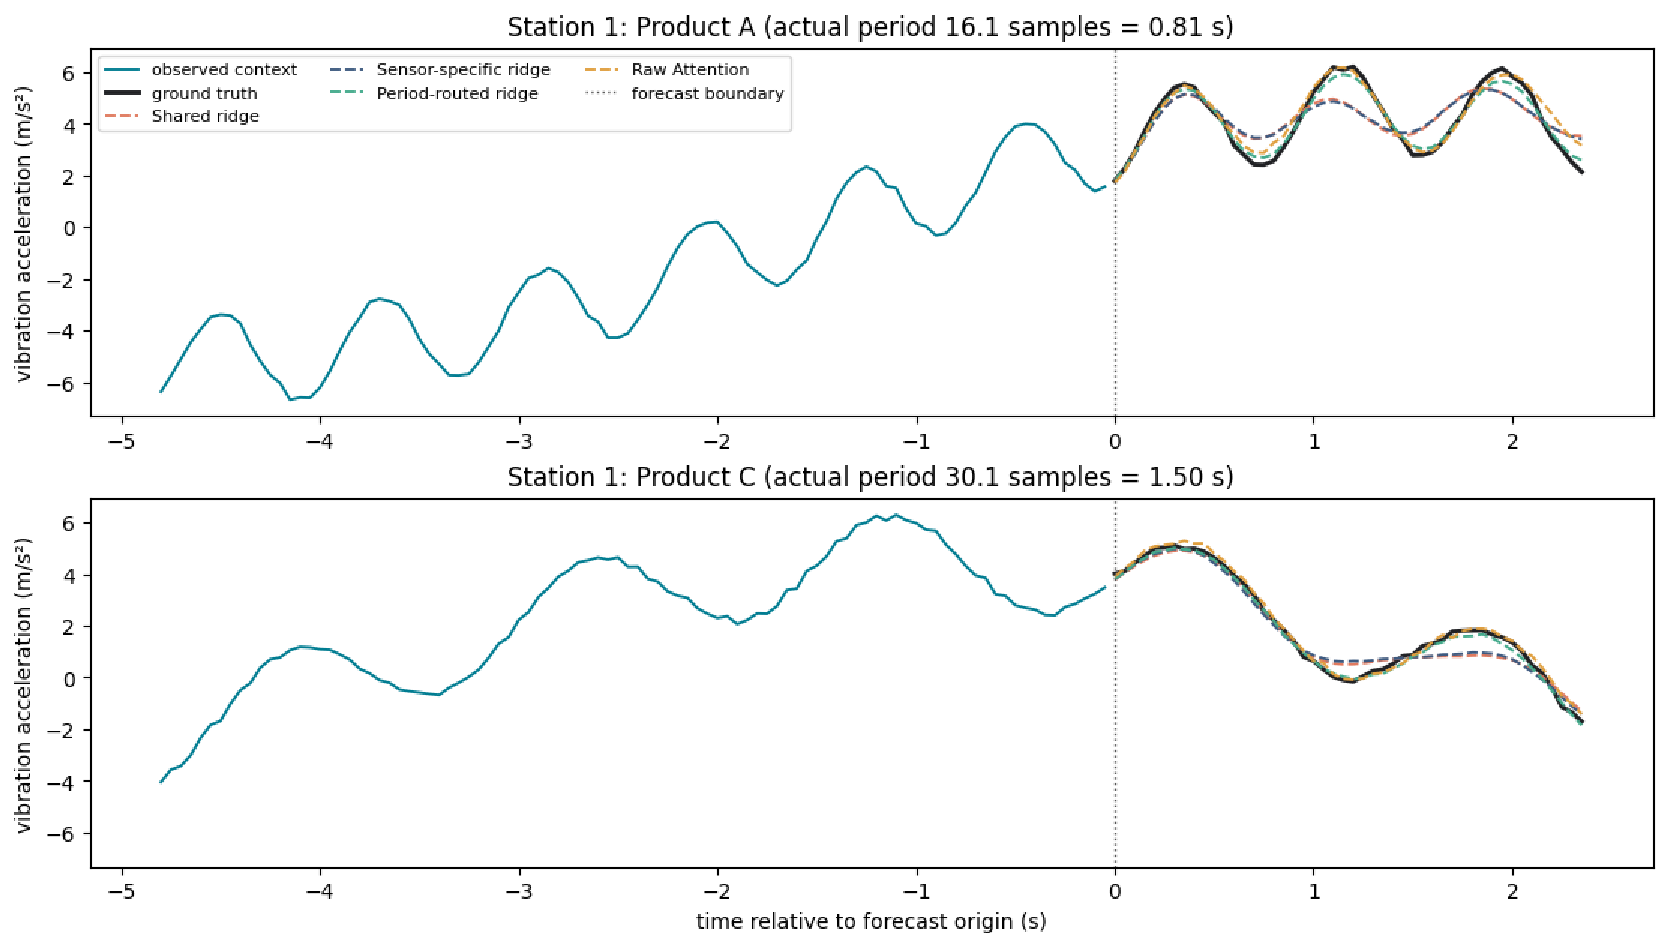
\includegraphics[width=0.83\linewidth]{figures/fig01_output1-2_regime_forecasts.pdf}
\caption{\label{fig:f1}Output 1.2 --- Station 1 under Product A ($P\!=\!16.1$) and Product C ($P\!=\!30.1$), validation.}
\end{figure}
\begin{itemize}
\item \textbf{The compromise is visible as damping.} For Product A the shared and sensor-specific ridge forecasts have the right rhythm but a shrunken amplitude (peaks $\approx$5 vs $\approx$6.2, troughs $\approx$3.5 vs $\approx$2.5); for Product C they flatten the second bump ($\approx$0.8 vs 1.8). Window RMSE: shared ridge 0.779 (A) and 0.448 (C) vs period-routed 0.232 and 0.150.
\item \textbf{Reason.} $\hat z=x^\top\widehat W$ applies one fixed weighting of past samples. Paces 14--36 need different phase advances; least squares averages them, and averaging waves with different phase advances cancels part of their amplitude.
\end{itemize}

\begin{figure}[H]\centering
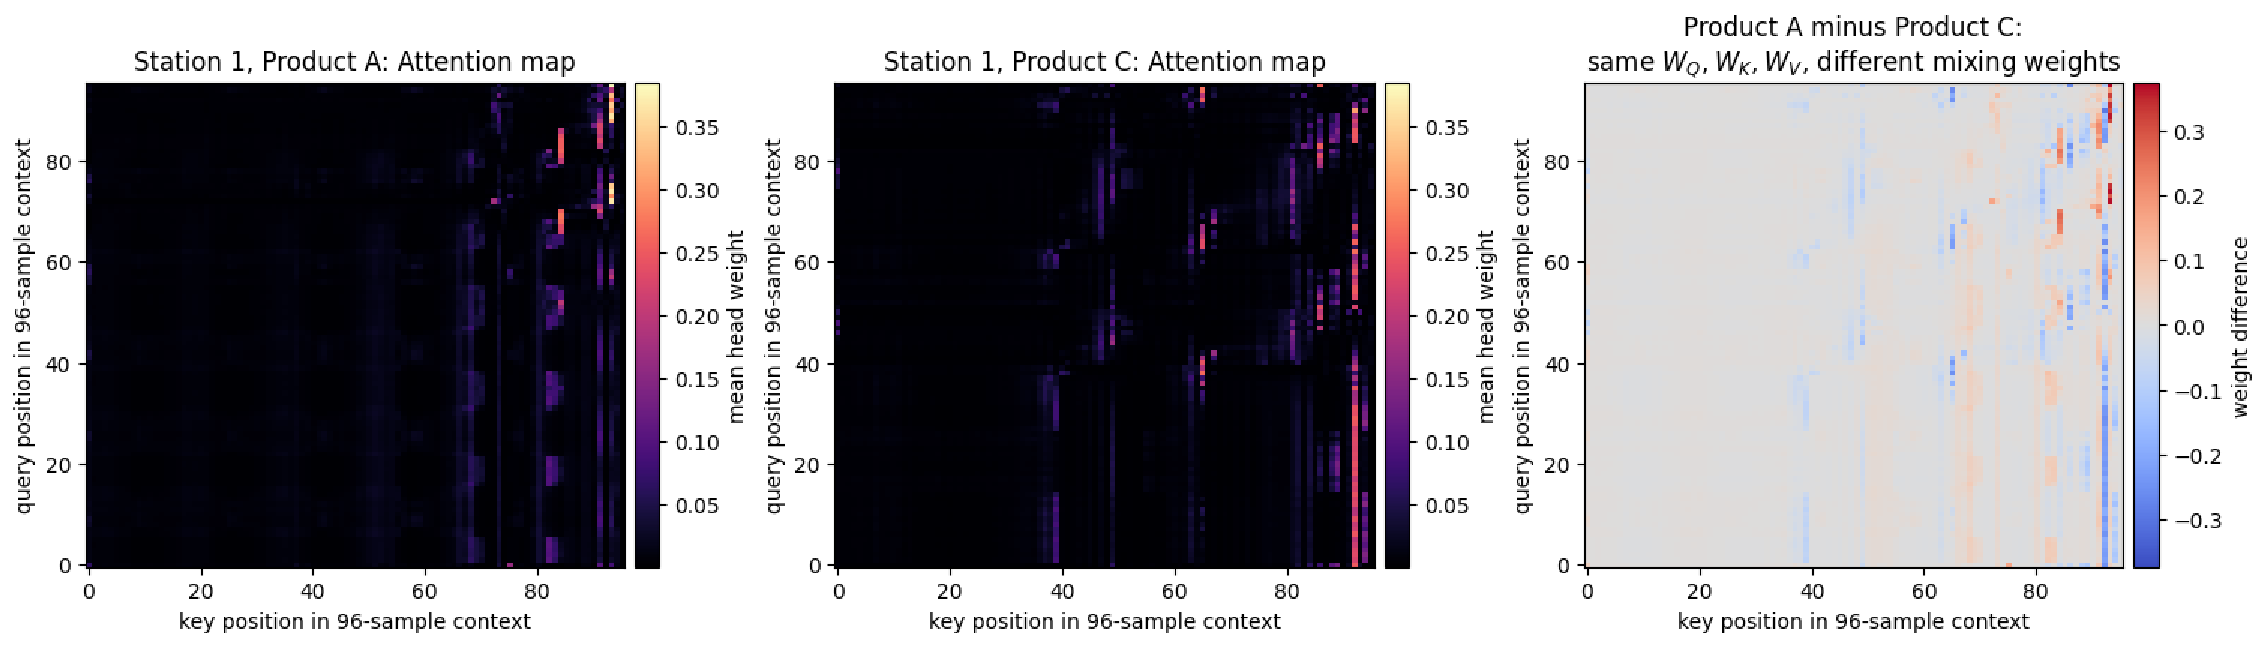
\includegraphics[width=0.95\linewidth]{figures/fig02_output1-3_attention.pdf}
\caption{\label{fig:f2}Output 1.3 --- Raw Attention maps for the two Station 1 contexts and their difference (validation).}
\end{figure}
\begin{itemize}
\item $W_Q,W_K,W_V$ are identical for both contexts, yet the weights differ by 0.012 on average and up to 0.373: the scores $QK^\top$ are recomputed from each window, so each context builds its own value-mixing matrix. Ridge instead applies the same $\widehat W$ to every window.
\item Both maps concentrate on recent keys (positions $\approx$65--95) in vertical stripes whose positions differ between the two contexts. This shows context-dependent mixing only; it is \emph{not} evidence that Attention recovered the physical period.
\end{itemize}

%---------------------------------------------------------------------
\subsection*{Response 2 --- separating slow structure from repetition}

\begin{figure}[H]\centering
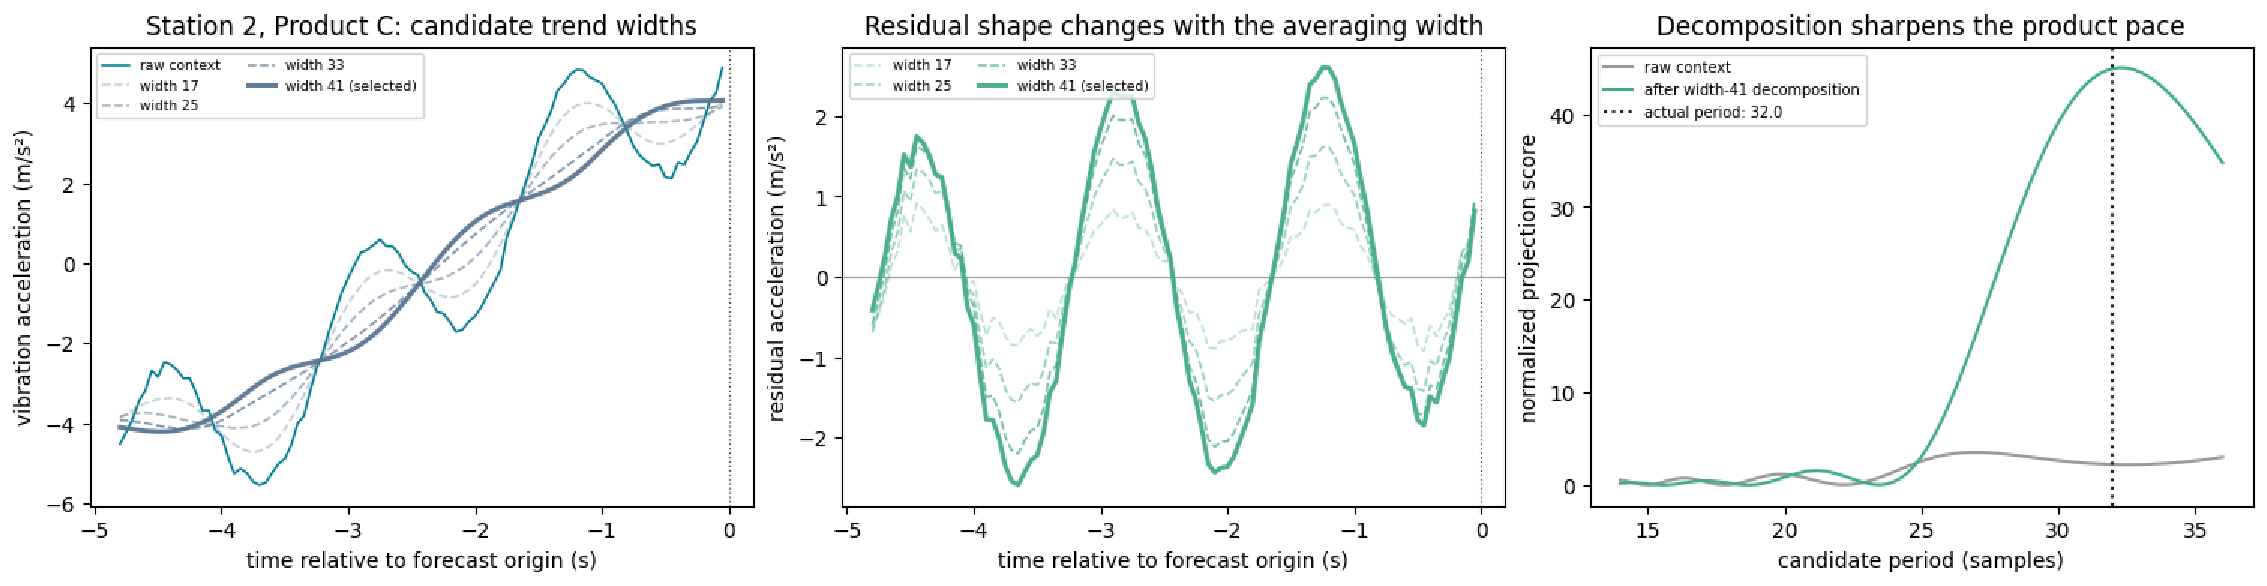
\includegraphics[width=0.95\linewidth]{figures/fig03_output2-1_decomposition.pdf}
\caption{\label{fig:f3}Output 2.1 --- candidate widths on one context (Station 2, Product C, validation).}
\end{figure}

\begin{table}[H]\centering\small
\caption{Output 2.2 (training-only oracle diagnostic) and Output 2.3 (validation RMSE).}
\begin{tabular}{lccccc}\toprule
Representation & raw & $m=17$ & $m=25$ & $m=33$ & $m=41$ (selected)\\\midrule
Period recovered within 1 sample & 0.687 & 0.980 & 0.989 & 0.993 & \textbf{0.998}\\
Median $|$period error$|$ (samples) & 0.525 & 0.157 & \textbf{0.122} & 0.142 & 0.216\\
Residual std in Output 2.1 (m/s$^2$) & -- & 0.578 & 1.012 & 1.372 & 1.572\\\bottomrule
\end{tabular}\\[6pt]
\begin{tabular}{lcccc|cccc}\toprule
& \multicolumn{4}{c|}{Established} & \multicolumn{4}{c}{Held-out}\\
Model & All & A & B & C & All & A & B & C\\\midrule
Raw Attention & 0.427 & 0.424 & 0.448 & 0.407 & 0.667 & 0.707 & 0.629 & 0.662\\
Attention + decomposition & \textbf{0.313} & 0.293 & 0.359 & 0.282 & \textbf{0.456} & 0.401 & 0.523 & 0.435\\\bottomrule
\end{tabular}\end{table}

\begin{itemize}
\item \textbf{Selected width $m=41$.} Visually (Fig.~\ref{fig:f3}), narrow widths ($m=17$) let the trend follow the vibration and shrink the remainder (std 0.58); $m=41$ gives a smooth ramp and a full-amplitude, centred remainder (std 1.57). After decomposition the projection score peaks sharply at the true period (32), which the raw context does not show. Near the right edge the replicated values flatten the trend.
\item \textbf{Empirically}, decomposition lifts oracle period recovery from 68.7\% to 99.8\% (training) and cuts Raw Attention's validation RMSE by 27\% on established (0.427$\to$0.313) and 32\% on held-out (0.667$\to$0.456), for every product. Note the criterion matters: $m=25$ has the smallest \emph{median} period error.
\item \textbf{Why a moving average fits this world.} The drift time scale (240 samples) is far from the vibration (14--36); averaging over $\gtrsim$ one cycle cancels the sinusoid but barely changes the drift, so $T\approx$ drift and $S\approx$ vibration $+$ noise. The \textbf{training-only oracle} measures directly what the width is meant to achieve (visible repetition), uses no validation/test data, and the true period is never given to the model, so selection is leak-free.
\item \textbf{Failure case / alternative.} An abrupt level shift (e.g.\ a recalibration step) is smeared into a ramp: part goes to $T$, and a spurious bump to $S$. Alternative: per-window linear detrending, which assumes a \emph{straight-line} trend inside the window; it is cheaper and edge-free but would leak the drift's curvature into $S$.
\end{itemize}

%---------------------------------------------------------------------
\subsection*{Response 3 --- mixing by temporal delay}

\texttt{aggregate\_delays} reproduces the worked example $[35,15,25,25]$ and passes the gradient check; \texttt{delay\_scores} matches the direct correlation $[4,-4,4,-4]$ (Output 3.1).

\begin{figure}[H]\centering
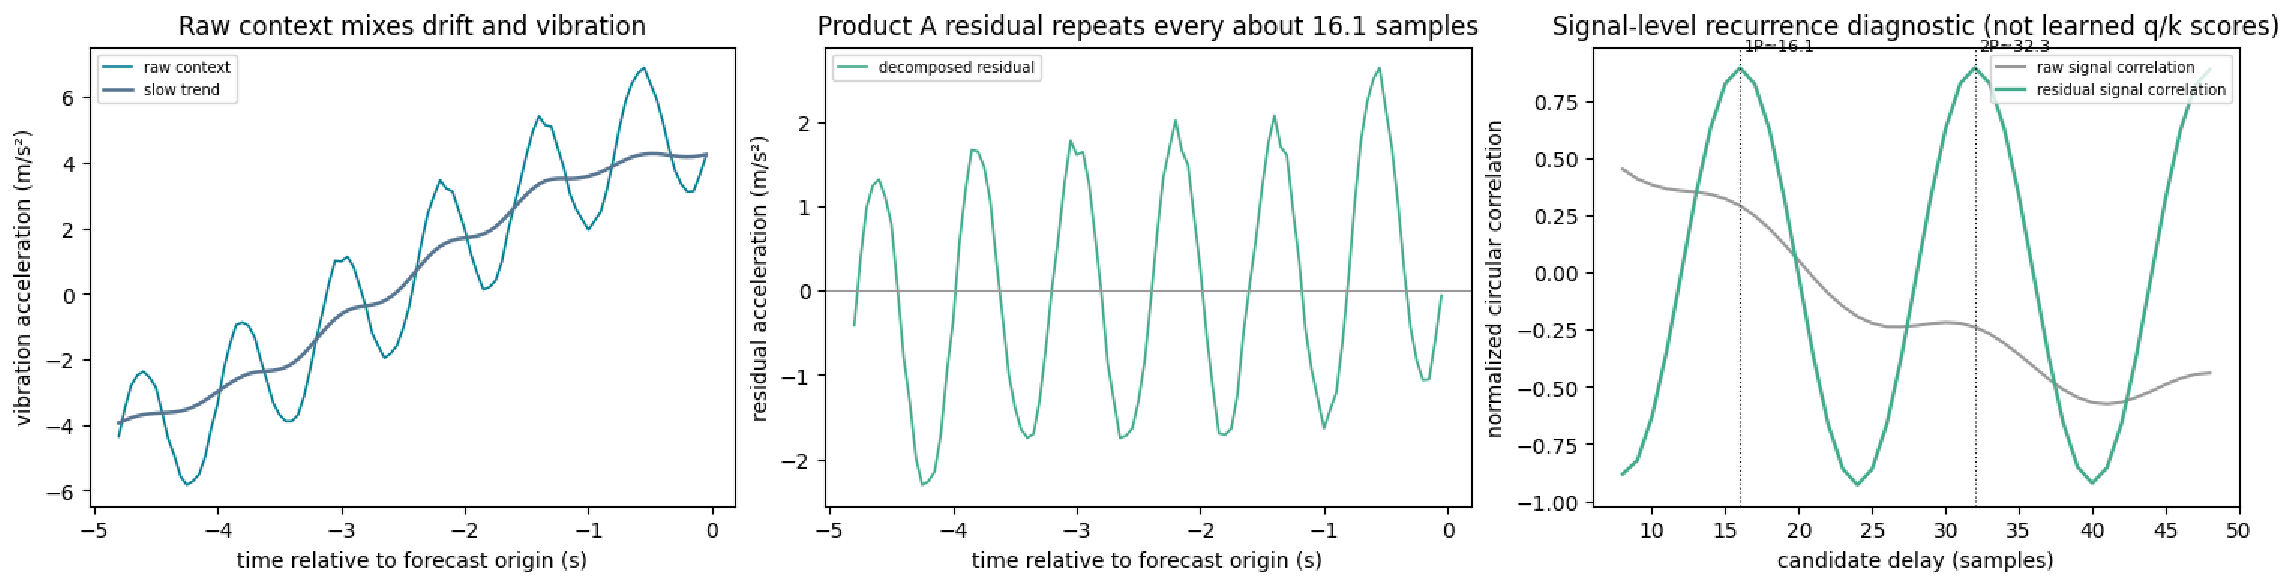
\includegraphics[width=0.95\linewidth]{figures/fig04_output3-2_recurrence.pdf}
\caption{\label{fig:f4}Output 3.2 --- signal-level recurrence diagnostic, Station 2, Product A ($P=16.135$), validation. Not learned q/k scores.}
\end{figure}
\begin{itemize}
\item \textbf{Strongest lags:} 16 and 32 (correlation 0.896 and 0.897), i.e.\ $P$ and $2P$ rounded to integers; the troughs at $\approx$24 and $\approx$40 ($\approx-0.9$) are half-period offsets $1.5P$ and $2.5P$. $3P\approx48$ sits at the band edge.
\item \textbf{Why decomposition cleans the evidence.} The raw correlation falls monotonically from $\approx$0.45 and has no peak at $P$: a ramp is similar to itself at every shift, which lifts all lags and hides the period. After removing the trend, peaks align with peaks only at multiples of $P$. The delay mixer scores exactly this kind of correlation (on learned features), so a trend-free input makes its top-$K$ selection land on the useful delays.
\item \textbf{When the assumption is wrong.} A period that drifts quickly inside one context (the machine ramping up speed): a lag of 16 matches the start of the window but not its end, and one shared set of $K$ delays per example cannot follow the change; it blends mismatched copies and smears the forecast. Isolated transients (a single knock) have no recurring lag at all; circular shifting can even wrap a spike from the end to the start.
\end{itemize}

%---------------------------------------------------------------------
\subsection*{Response 4 --- compare designs and deploy}

\textbf{(a) Prediction (before Output 4.1)} \fix{confirm this was your own prediction}: decomposition should help most where the slow component is prominent, because it removes the ramp before mixing, while a delay mixer on raw input scores lags on a ramp that correlates with itself at every shift.

\begin{table}[H]\centering\small
\caption{Outputs 4.1 and 4.3 --- validation RMSE (MSE) in m/s$^2$ ((m/s$^2$)$^2$); cost.}
\begin{tabular}{lcccrr}\toprule
Model & Established & Held-out & Est.\ A / B / C & Params & Fit (s)\\\midrule
Raw Attention & 0.427 (0.182) & 0.667 (0.444) & 0.424 / 0.448 / 0.407 & 368{,}368 & 65.8\\
Raw delay mixer & 0.231 (0.053) & 0.332 (0.110) & 0.212 / 0.216 / 0.262 & 368{,}370 & 87.2\\
Attention + decomposition & 0.313 (0.098) & 0.456 (0.208) & 0.293 / 0.359 / 0.282 & 373{,}024 & 86.8\\
Autoformer-inspired & \textbf{0.199} (0.039) & \textbf{0.244} (0.059) & 0.224 / 0.184 / 0.185 & 373{,}026 & 107.3\\\midrule
Shared ridge & 0.767 (0.588) & 0.876 (0.767) & 0.805 / 0.854 / 0.621 & 4{,}608 & 0.003\\
Period-routed ridge & \textbf{0.166} (0.028) & \textbf{0.173} (0.030) & 0.181 / 0.164 / 0.152 & 59{,}904 & 0.013\\\midrule
\multicolumn{6}{l}{\emph{Test} (Output 4.3, chosen model): period-routed ridge 0.161 established, 0.183 held-out.}\\\bottomrule
\end{tabular}\end{table}

\begin{figure}[H]\centering
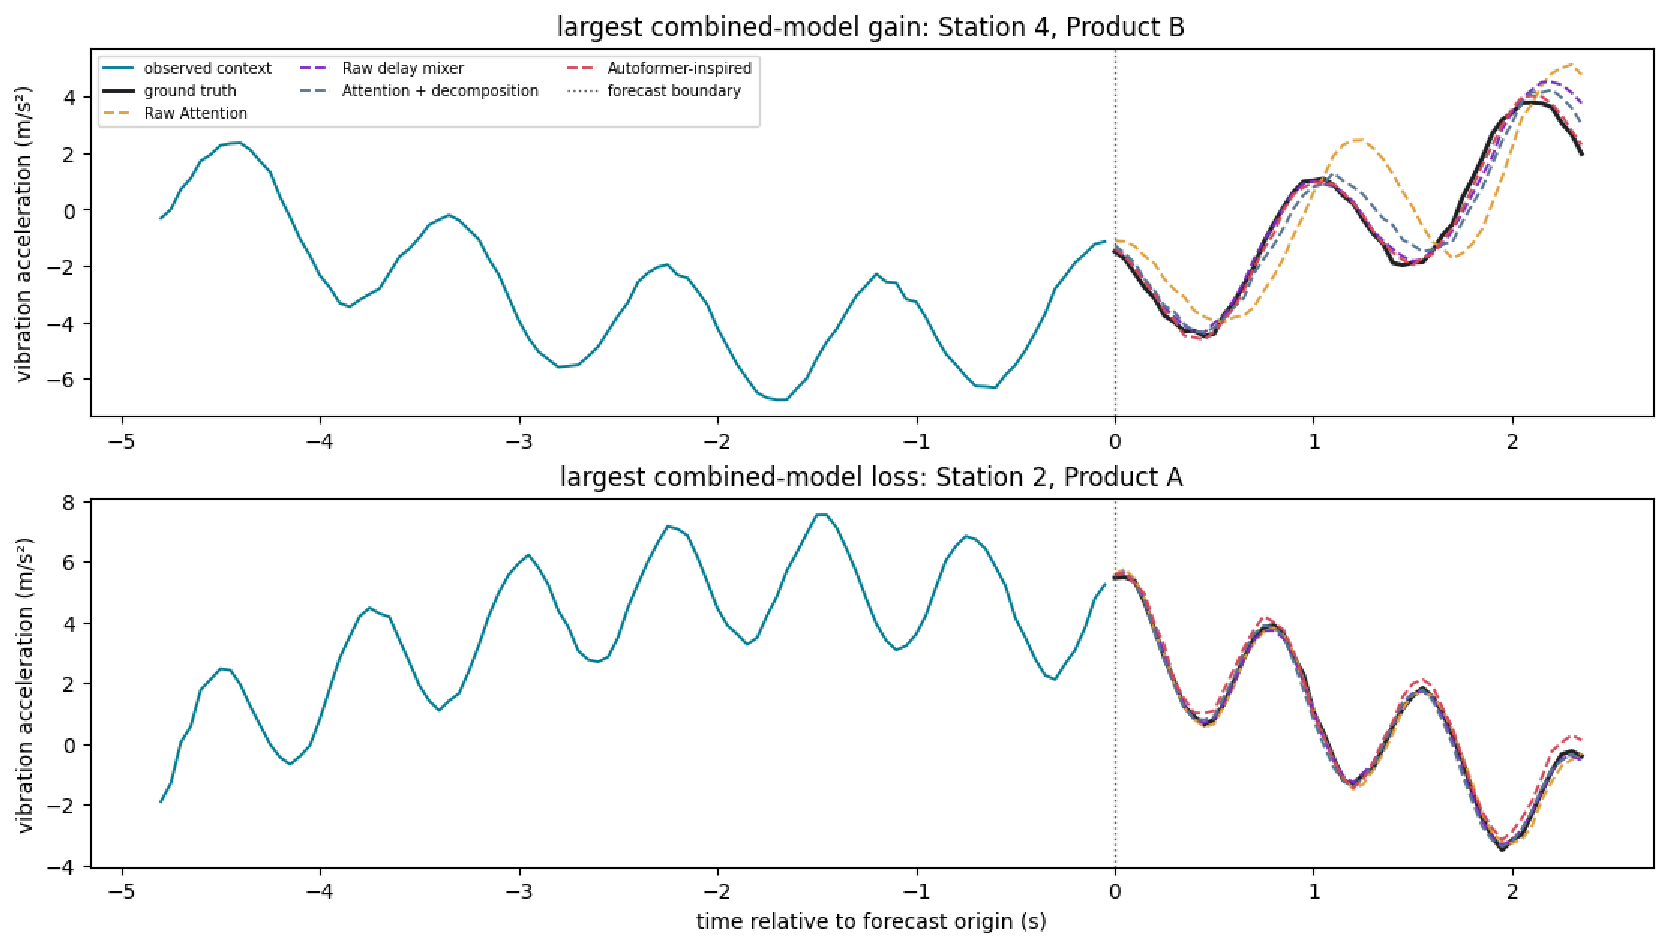
\includegraphics[width=0.72\linewidth]{figures/fig05_output4-1_contrasting_cases.pdf}
\caption{Output 4.1 contrasting cases (validation). Largest combined-model gain: Station 4, Product B (window RMSE Raw Attention 1.670, Autoformer-inspired 0.197; Raw Attention lags in phase). Largest loss: Station 2, Product A (0.174 vs 0.301).}\label{fig:f5}
\end{figure}

\begin{figure}[H]\centering
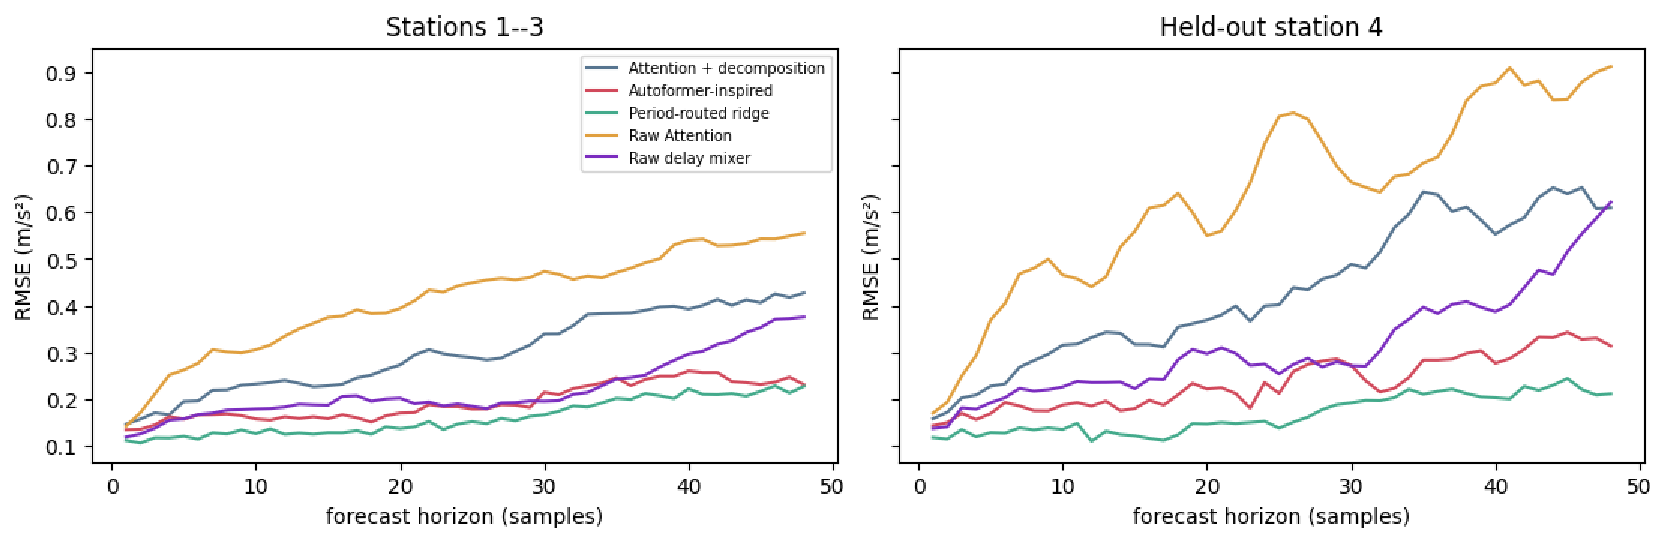
\includegraphics[width=0.78\linewidth]{figures/fig06_output4-2_horizon.pdf}
\caption{\label{fig:f6}Output 4.2 --- validation RMSE by horizon step.}
\end{figure}

\textbf{(b) Interpretation} (established validation MSE unless stated).
Both switches help in both settings. Delay mixing: $0.182\to0.053$ on raw input and $0.098\to0.039$ on decomposed input. Decomposition: $0.182\to0.098$ with Attention and $0.053\to0.039$ with delay mixing. Delay mixing is the larger upgrade. The gains overlap: separately they save $0.084+0.129=0.213$, together $0.143$ (held-out: $0.570$ vs $0.385$), consistent with both addressing the same drift-plus-repetition structure; this run shows the overlap, not its cause. Errors grow with horizon for every model (Fig.~\ref{fig:f6}): Raw Attention rises fastest (established $\approx$0.15$\to$0.55, held-out $\to$0.9), Autoformer-inspired stays close to period-routed ridge on established ($\approx$0.13$\to$0.23 vs 0.11$\to$0.23) but reaches $\approx$0.31 on held-out.

\textbf{(c) Deployment} (rule fixed before Output 4.3: lowest validation RMSE; prefer a cheaper model within 2\%).
\emph{Established:} period-routed ridge, with the lowest validation RMSE (0.166), 6$\times$ fewer parameters and a 0.013\,s fit versus 107\,s. \emph{Held-out:} period-routed ridge (0.173 vs 0.244); it never uses station identity. Test (0.161, 0.183) confirms it. Caveat: it depends on a hand-built period estimator; the best learned alternative is Autoformer-inspired.

\clearpage
%=====================================================================
\section*{Task 2 --- Leaderboard challenge (Autoformer)}

\textbf{Final submission (v2):} leaderboard RMSE \textbf{81.11}, MAE 53.01, sMAPE 49.94\%, $P=446{,}085$, $E=105$, score 81.1656 (2nd at the time of writing). First submission (v1): RMSE 99.09, $P=120{,}645$, $E=75$. Code: \texttt{Task2/task2\_v1\_experiments.ipynb} (all experiments and ablations), \texttt{Task2/task2\_v2\_final.ipynb} (final model). $P$ and $E$ are printed by the notebooks and saved in \texttt{Task2/results/submission\_meta\_v*.json}.

\subsection*{1. Data and exploratory analysis}
\begin{itemize}
\item 43{,}656 values, non-negative, heavy-tailed: median 73, mean 98, 99th percentile 418, max 994, skewness 1.83.
\item \textbf{Short memory:} autocorrelation 0.97 (lag 1), 0.40 (24), 0.16 (48), 0.03 (168). The target's own past says little about most of a 168-step horizon.
\item \textbf{Period recovered without timestamps:} periodogram peak (periods 8--60) = 24 and ACF of first differences peaks at 24; the raw ACF decays monotonically, so its maximum is not usable. The daily profile is mild (86--113); there is no clear weekly pattern (Fig.~\ref{fig:f7}). The period sets the moving-average width (25) and phase features.
\item \textbf{External variables} (six continuous, four mutually exclusive binary): simultaneous correlation with $\log(1+y)$ up to $|0.35|$ (A $+0.31$, D $-0.35$, H $-0.35$, I $+0.23$). Several correlate more strongly 6 steps earlier (H $-0.43$, I $+0.31$), which suggests accumulation effects; this motivated trailing-mean features.
\end{itemize}
\begin{figure}[H]\centering
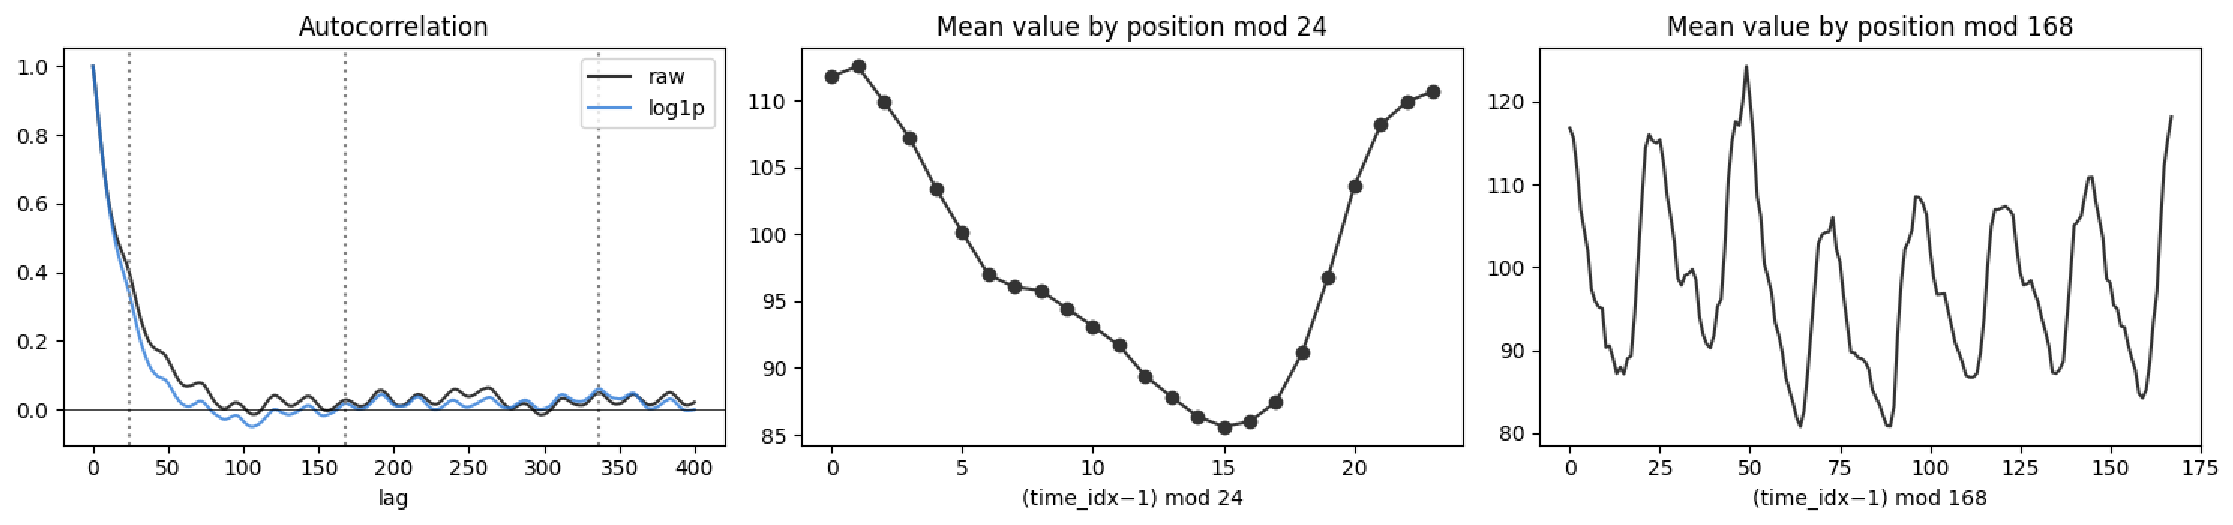
\includegraphics[width=0.9\linewidth]{figures/fig07_task2_memory_period.pdf}
\caption{\label{fig:f7}Autocorrelation, and mean value by position mod 24 and mod 168 (training history).}
\end{figure}

\subsection*{2. Validation protocol}
\begin{itemize}
\item Chronological \textbf{rolling origin}: training targets in $[0, 39288)$; evaluation on the last \textbf{26 non-overlapping 168-step weeks}. Scalers fitted on the training region only.
\item Every configuration is run with \textbf{3 seeds} (5 in v2); results are mean $\pm$ std over seeds, plus \textbf{paired per-week differences} for with/without comparisons.
\item \textbf{Epochs as a hyper-parameter:} after every epoch the model forecasts all evaluation weeks; the epoch count with the best mean is used, fixed, when refitting on all data. An 8-week early-stopping split was tried first and disagreed with the 26-week estimate (too noisy).
\item RMSE, MAE and sMAPE are tracked for every run. Naive baselines on the 26 weeks (RMSE / MAE / sMAPE): last-week mean 82.8 / 68.2 / 79.5; seasonal naive (24) 106.6 / 84.5 / 94.2; persistence 115.4 / 95.5 / 88.3.
\end{itemize}

\subsection*{3. Preprocessing, features and architecture}
\begin{itemize}
\item \textbf{Target:} \texttt{log1p} or raw, then standardised; forecasts inverted and clipped at 0.
\item \textbf{Covariates:} $\log(1+\cdot)$ on skewed D, E, F; continuous features standardised; binary one-hot kept as 0/1; sin/cos phase features for periods 24 and 168 (from \texttt{time\_idx} only); optional trailing means over 6/24/72 steps (use only values up to $t$, available across the horizon because the file covers it).
\item \textbf{Where external data enters:} \texttt{none} (phase only); \texttt{past} (external in the encoder only); \texttt{full} (external also in the decoder, including the 168 known future steps); \texttt{full+roll} (plus trailing means). Covariates enter through a linear embedding added to the value embedding, in place of Autoformer's timestamp embedding.
\item \textbf{Autoformer} (Wu et al., 2021; structure follows github.com/thuml/Autoformer; written from scratch): encoder--decoder, input 336, label 168, horizon 168 (direct, no recursion). \emph{Series decomposition}: replicate-padded moving average (width 25), applied to the input and after every sub-layer; the decoder accumulates the extracted trends. \emph{Auto-Correlation}: FFT delay scores averaged over heads and channels, top $k=\lfloor \ln L\rfloor=5$ delays per example, softmax weights, aggregation of $v_{(t-\tau)\bmod L}$ (same convention as Task 1). $d_{\text{model}}=32$, 4 heads, 1+1 layers, $d_{ff}=64$ (24{,}129 parameters with \texttt{full+roll}); Adam, lr $3\!\times\!10^{-4}$ decayed $\times0.85$ per epoch, batch 128, training stride 4. Unit tests reuse the Task 1 worked examples.
\end{itemize}

\subsection*{4. Experiment 1 (v1): target transform $\times$ external-data ablation, 3 seeds}
\begin{table}[H]\centering\small
\caption{Mean over seeds of the per-week metrics on the 26 evaluation weeks (seed std of RMSE in brackets).}
\begin{tabular}{llccccc}\toprule
Target & External data & RMSE & MAE & sMAPE (\%) & Params & Best epoch\\\midrule
log1p & full+roll & \textbf{55.35} (1.61) & \textbf{39.88} & \textbf{50.8} & 24{,}129 & 15\\
raw & full+roll & 61.44 (1.07) & 48.99 & 67.2 & 24{,}129 & 3\\
log1p & full & 62.97 (2.02) & 45.35 & 56.2 & 22{,}209 & 12\\
raw & full & 65.39 (1.76) & 53.71 & 70.7 & 22{,}209 & 11\\
raw & past & 80.85 (1.35) & 66.84 & 78.9 & 21{,}889 & 4\\
raw & none & 81.22 (0.81) & 67.90 & 79.3 & 21{,}569 & 4\\
log1p & none & 82.49 (0.69) & 63.29 & 80.0 & 21{,}569 & 10\\
log1p & past & 83.13 (0.39) & 63.86 & 80.7 & 21{,}889 & 2\\\midrule
\multicolumn{2}{l}{Baseline: mean of last 168} & 82.80 & 68.21 & 79.5 & -- & --\\\bottomrule
\end{tabular}\end{table}

\begin{table}[H]\centering\small
\caption{Paired per-week differences in RMSE (negative = first variant better), 26 weeks $\times$ 3 seeds.}
\begin{tabular}{llccc}\toprule
Target & Comparison & Mean $\Delta$RMSE & Std.\ error (weeks) & Weeks improved\\\midrule
log1p & full $-$ none & $-19.5$ & 4.2 & 88\%\\
log1p & past $-$ none & $+0.6$ & 0.2 & 31\%\\
log1p & full+roll $-$ full & $-7.6$ & 2.3 & 81\%\\
raw & full $-$ none & $-15.8$ & 4.2 & 77\%\\
raw & past $-$ none & $-0.4$ & 1.2 & 46\%\\
raw & full+roll $-$ full & $-4.0$ & 1.9 & 65\%\\\bottomrule
\end{tabular}\end{table}

\begin{figure}[H]\centering
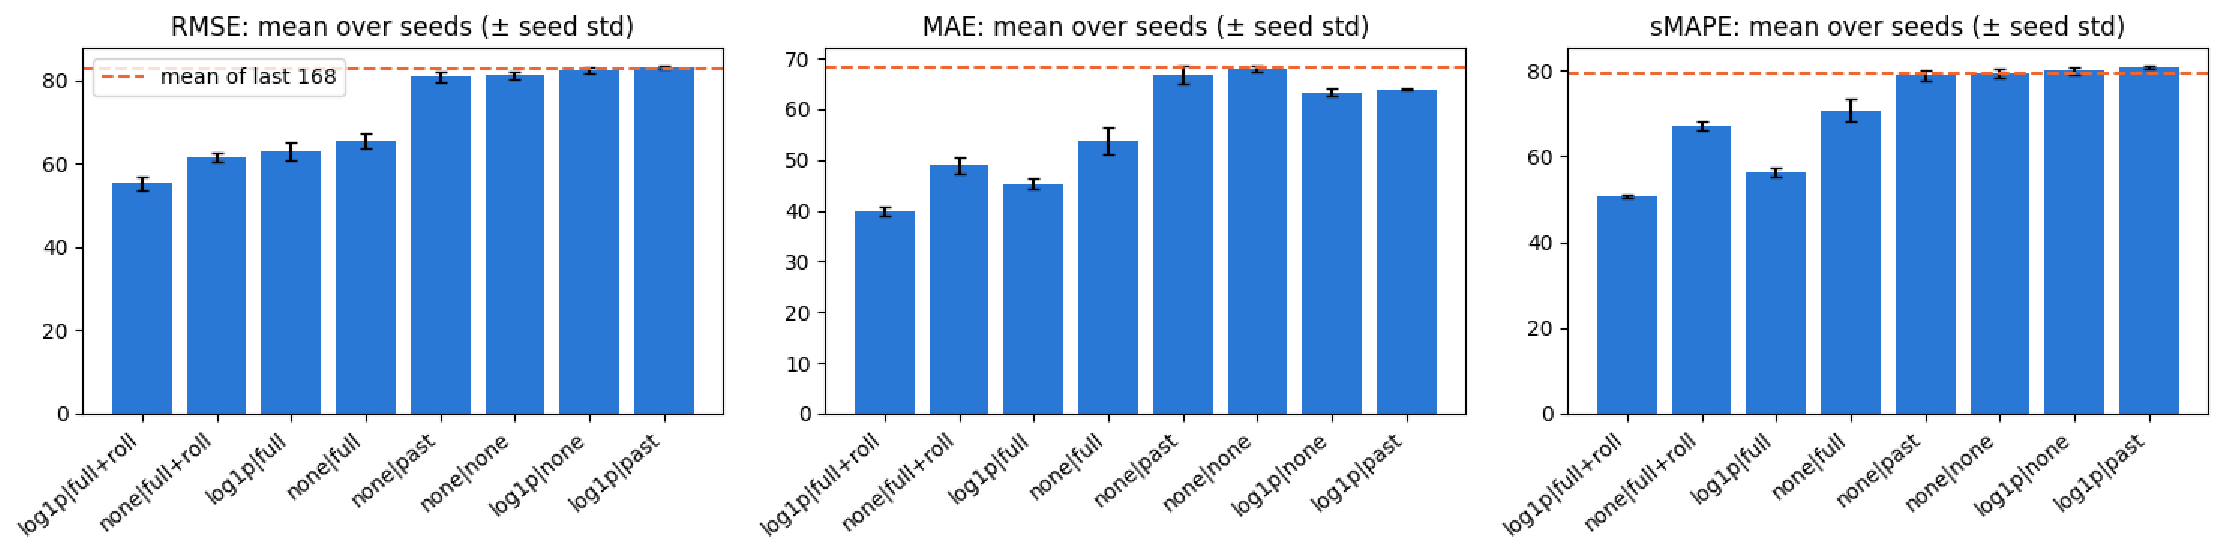
\includegraphics[width=0.95\linewidth]{figures/fig08_task2_exp1_ablation.pdf}
\caption{\label{fig:f8}Experiment 1: RMSE, MAE and sMAPE per configuration (mean $\pm$ seed std); dashed line = last-week-mean baseline.}
\end{figure}

\textbf{Findings (external-data ablation).}
\begin{itemize}
\item \textbf{The optional file helps only through its future part.} Adding it to the encoder only (\texttt{past}) changes nothing ($+0.6$ / $-0.4$, within noise); adding the known future values to the decoder cuts RMSE by 16--20 and wins in 77--88\% of weeks. Trailing means add another 4--8. This matches their timing: the future covariates carry information about the horizon that the target's short memory cannot.
\item \textbf{Occlusion} (inputs replaced by train means at evaluation, no retraining, best \texttt{full} models): all external data $+36$ RMSE (log) / $+23$ (raw), almost all from the \emph{future} portion ($+36$ / $+28$) vs past ($+7$ / $+8$). By variable: A ($+22$ / $+18$) and B ($+11$ / $+15$) dominate, then H ($+7$ / $+4$) and J ($+5$ / $+1$); every other variable adds $\le3$.
\item \textbf{Without external data no model beats the naive baseline} (80.9--83.1 vs 82.8): the series' own history is not enough at a 168-step horizon.
\item \textbf{Metric disagreement.} log1p wins most clearly on MAE and sMAPE (relative accuracy on low values), less so on RMSE, which is dominated by spikes that a log-target model under-predicts.
\item \textbf{Model size} (log1p, full+roll): $d=16$: 61.4; $d=32$: 55.3; $d=64$: 57.2 (lowest seed spread, 0.5); $d=64$, 2+2 layers: 57.4. Larger models did not pay for themselves on the 26-week average.
\end{itemize}

\subsection*{5. From v1 to v2: why the first leaderboard score was worse than validation}
v1 (5-seed ensemble of \texttt{log1p|full+roll}, 15 epochs) scored RMSE 99.09 on the leaderboard, versus $\approx$55--59 on validation. Per-week statistics explain the gap: the last 12 evaluation weeks, right before the leaderboard week, are a different regime (mean 109 vs 73, std 101 vs 46, typical maximum 388 vs 207); even the naive baseline has RMSE 111.6 there vs 58.1 on the earlier weeks (Fig.~\ref{fig:f9}). The 26-week average was dominated by calm weeks.

\begin{figure}[H]\centering
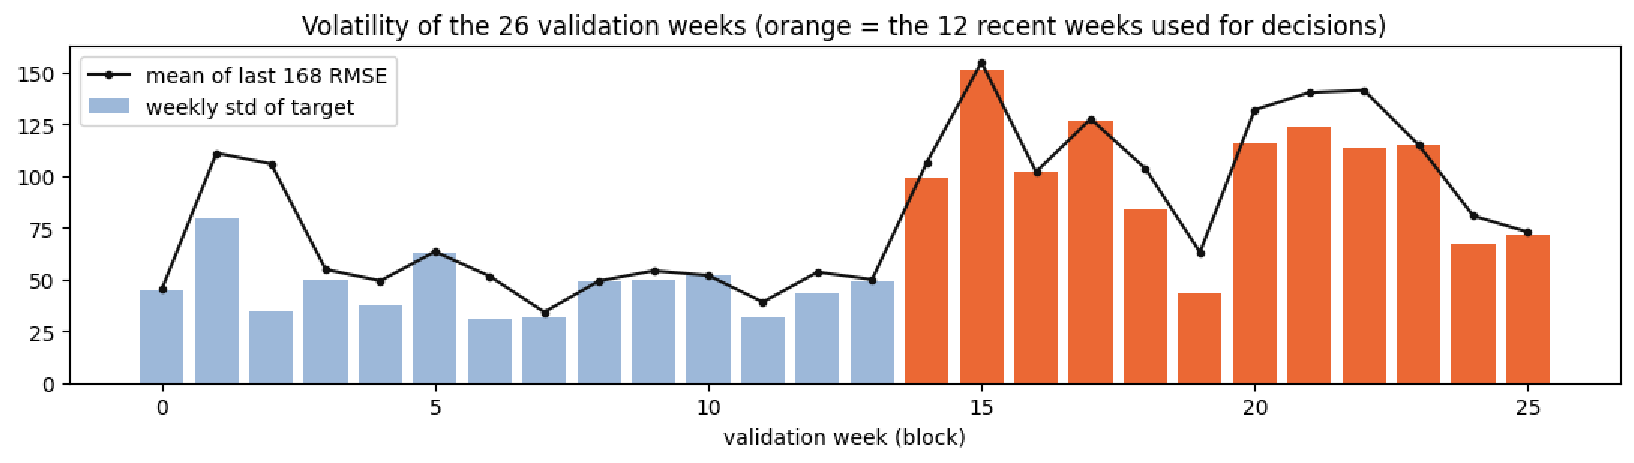
\includegraphics[width=0.85\linewidth]{figures/fig09_task2_week_volatility.pdf}
\caption{\label{fig:f9}Weekly standard deviation of the target and baseline RMSE for the 26 evaluation weeks (orange = recent 12).}
\end{figure}

\textbf{v2 protocol.} Decisions on the \textbf{recent 12 weeks}; three candidates $\times$ 5 seeds, up to 25 epochs; the seed-ensemble is scored after each epoch. A blend $s\,(w\,\text{LOG}+(1-w)\,\text{RAW})$ was evaluated by \textbf{leave-one-week-out} cross-validation (choose $w,s$ on 11 weeks, score the 12th).

\begin{table}[H]\centering\small
\caption{Recent-12-week and all-26-week RMSE of seed ensembles (v2).}
\begin{tabular}{lcc}\toprule
Recipe & Recent 12 weeks & All 26 weeks\\\midrule
Naive baseline (mean of last 168) & 111.64 & 82.80\\
v1 recipe (log1p, $d=32$, epoch 15) & 66.67 & 53.95\\
LOG only: log1p, $d=64$, epoch 21 & 64.13 & 52.44\\
RAW only: raw, $d=32$, epoch 4 & 77.63 & 59.51\\
50/50 blend & 68.17 & 53.08\\
\textbf{Tuned: $w=1$, $s=1.2$ (leave-one-week-out)} & \textbf{63.27} & 50.19\\\bottomrule
\end{tabular}\end{table}

\begin{figure}[H]\centering
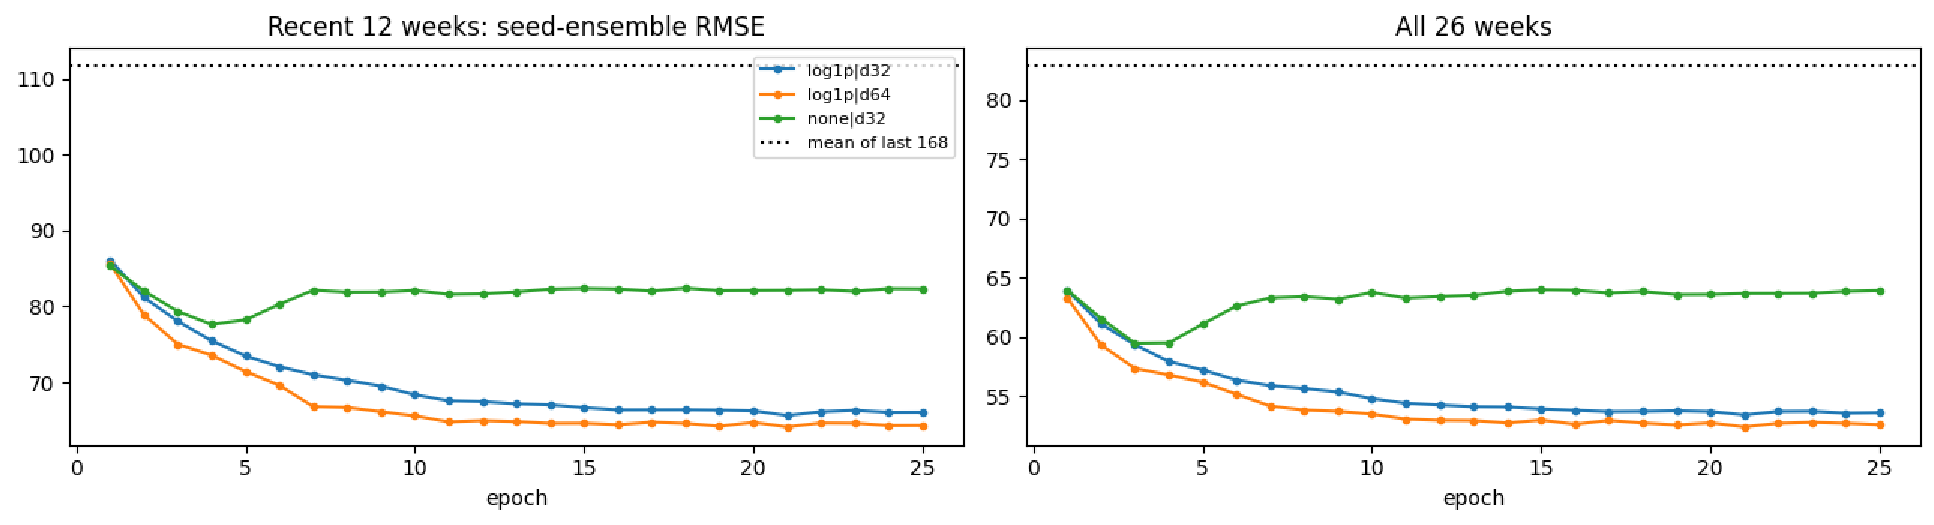
\includegraphics[width=0.9\linewidth]{figures/fig10_task2_v2_epoch_curves.pdf}
\caption{\label{fig:f10}v2: seed-ensemble RMSE after each epoch, recent 12 weeks and all 26 weeks.}
\end{figure}
\begin{itemize}
\item \textbf{Ensembling matters:} single-seed recent RMSE $\approx$71--73 vs 64--66 for the 5-seed average.
\item \textbf{Blending with the raw-target model hurt}; the selected recipe is the wider log model scaled by $s=1.2$, which corrects the log model's downward bias (back-transforming a mean of logs gives a median-like forecast). Out of sample it improved the recent-week RMSE from 66.7 (v1 recipe) to 63.3.
\item \textbf{Final model:} 5 seeds of \texttt{log1p}, full+roll, $d=64$, trained on all data for 21 epochs each, averaged and scaled by 1.2: $P=5\times89{,}217=446{,}085$, $E=5\times21=105$. The forecast has the same shape as v1 (correlation 0.99) at a 38\% higher level (Fig.~\ref{fig:f11}).
\item \textbf{Leaderboard:} RMSE 99.09 $\to$ 81.11, MAE 63.6 $\to$ 53.0, sMAPE 54.3\% $\to$ 49.9\%. This is a single-week check; the decision was made from the cross-validated table above.
\end{itemize}

\begin{figure}[H]\centering
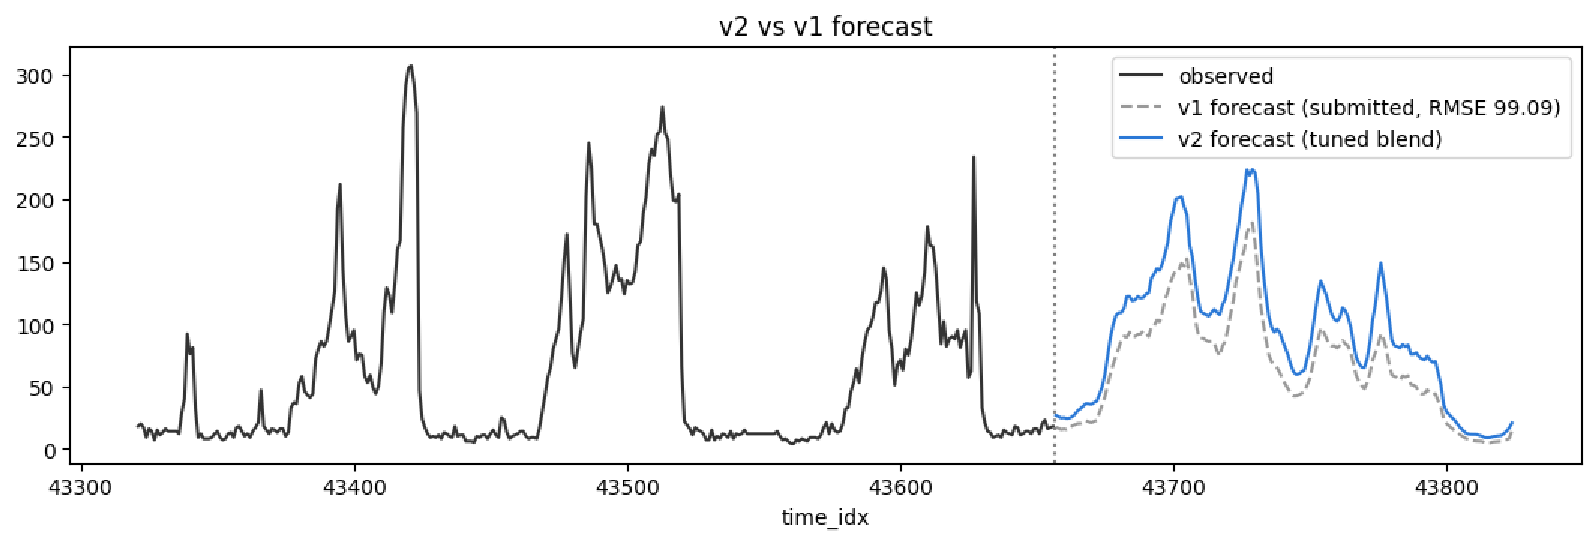
\includegraphics[width=0.9\linewidth]{figures/fig11_task2_final_forecast.pdf}
\caption{\label{fig:f11}Final v2 forecast (blue) vs the first submission v1 (dashed), with the last two observed weeks.}
\end{figure}

\subsection*{6. Leaderboard penalty and limitations}
\begin{itemize}
\item Fitting score $-$ RMSE against $P$ and $E$ for the published rows gives $\alpha\approx1.9\times10^{-9}$ and $\beta\approx5.0\times10^{-4}$; both our submissions matched the prediction (0.0377 and 0.0534). Accuracy dominates the score, which justified 5-seed ensembles.
\item \textbf{Limitations.} Epoch counts and $s$ were chosen on the same evaluation weeks that report them (the leave-one-week-out value is the honest one for $s$); 12 weeks is a small sample of a heavy-tailed series; the remaining RMSE gap comes from under-predicted spikes. A loss that weights large values more, or a raw-scale loss on a log-parameterised output, is the next step.
\end{itemize}

%=====================================================================
\section*{Use of generative AI}
Claude (Anthropic) was used as a learning partner and coding assistant, as allowed by the course AI policy. \fix{fill in the ``My edits'' column, and adjust the prompt wording to what you actually typed}

\begin{small}
\begin{tabularx}{\linewidth}{>{\raggedright\arraybackslash}p{4.3cm}>{\raggedright\arraybackslash}X>{\raggedright\arraybackslash}p{3.4cm}}\toprule
Prompt (summary) & Output & My edits\\\midrule
``Explain what I have to do in this assignment, the problem statement and how we are solving it''; follow-ups on inductive bias, period, sensors, noise, even-width moving averages & Explanations of both tasks and of Parts 0--4; an interactive visualisation of the simulated production line & \fix{fill in}\\
``Give me the notebook solved according to the instructions; I will run it on Kaggle T4'' & The three Task 1 implementations, a Kaggle setup cell, a validation-only deployment-choice rule; the full Task 2 v1 notebook (EDA, validation protocol, Autoformer, ablations) & \fix{fill in}\\
Leaderboard rows shared: ``make the model such that the formula gives the best value'' & Estimate of $\alpha,\beta$; 5-seed ensembles, trailing-mean covariates, epoch selection on validation & \fix{fill in}\\
v1 leaderboard result (RMSE 99.09) and executed notebook & Diagnosis (volatile recent weeks) and the v2 notebook with leave-one-week-out blending/scaling & \fix{fill in}\\
``Give me all files needed to submit'' & Draft of this report, figure PDFs, repository README & \fix{fill in}\\\bottomrule
\end{tabularx}
\end{small}

\small\textbf{References.} Wu et al.\ (2021), Autoformer, NeurIPS; reference code github.com/thuml/Autoformer. Vaswani et al.\ (2017). Zeng et al.\ (2023). Hyndman \& Athanasopoulos, \emph{Forecasting: Principles and Practice}.

\end{document}
